\section{Experiments on unsupervised RL benchmark} 

Through the experiment, we show sample efficient training is possible only by adding trivial number of parameters(=skill-dim).
We experimented our methods on URLB ($https://github.com/rll-research/url_benchmark$) where unsupervised RL methods could be compared fairly and easily.

There are two phases in URLB.
First phas is a reward-free pretrain phase and the other is finetuning phase with explicit rewards.
In a reward-free environment, methods such as DIAYN tries to train the agent to learn something meaningful using intrinsic reward.
Through this pretrain phase, the agent learns some behavior and we call this behavior as skill.
The method we propose in this paper is a methodology on how to get a higher reward faster when finetuning the learned behavior.

DIAYN is fixed as the pretrain method and finetuning is performed in various ways.
To follow the comparison introduced in the CIC paper, 2 million steps are pretrained and then 100,000 steps finetuning is performed.
Our method outperformed the other pretrain-finetune methods in 12 environments and the result is summarized on table \cref{finetuning result}.
It is noteworthy that the simplest state agnostic skill weight method among our proposed methods obtained the best performance. 
However, we also introduce the results of other skill as perspective methods as mention in 3.Method.

\subsection{Simple trainable skill weight}
The first is to introduce several parameters which counts to skill dim.
These parameters are used to weight each skill using additional parameters as large as the skill dimension.
The parameters are trainined in end-to-end manner using DDPG which is a default finetuning method in URLB.
These parameters serve to fuse the state viewed from various perspectives to help the agent obtain the optimal reward in a faster way.

The input state will be transformed into using these parameters. 
$[s',z_i'] = \sum_{i}^{d}w_i [s,z_i]/d$
Then, the transformed state will be fed into policy network to generate an action.
$a \sim g(\phi_i(s)), \text{where} \phi_i=f([s',z_i'])$

\subsubsection{Comparison with vanilla DIAYN}
We compare the results of using our method and not using our method during Finetune When the pretrain method is both DIAYN.
The results were better than default DIAYN finetuning using DDPG update.

We believe this result came about for two reasons.
First, the default DIAYN finetune uses only one skill per episode.
This has disadvantage of not being able to utilize other skills learned during pretraining.
Secondly, the sampled skill is not optimal with high probability.
Since, there's no way default DIAYN finetuning know which skill is good for the downstream task,it samples the skill uniformly.
And this uniform sampling of course couldn't be optimal.
This may be useful if interpreted as a method of obtaining a general agent in multi-task learning,
but it is inappropriate as an approach that aim to achieve maximum performance in a specific goal-oriented downstream task.
On the other hand, our method utilizes all skills and learns how to use various skills harmoniously to achieve better performance.
In \cref*{final_skill_weight}, we can check the agent use skills near evenly.
This allows for faster and better performance, as shown in the \cref{walker-run-simple-weight}.

\begin{table}[t]
  \caption{Performance at finetuning}
  \label{finetuning result}
  \vskip 0.15in
  \begin{center}
  \begin{small}
  \begin{sc}
  \begin{tabular}{lcccr}
  \toprule
  Domain & Task & BASE DIAYN & Other best & Ours \\
  \midrule
  Walker & Flip    &  \\
   & Run    & 158$\pm$8 & 486$\pm$25 & 542\\
   & Stand    &  \\
   & Walk    &  \\
  Quadruped & Jump    &  \\
   & RUn    &  \\
   & Stand    &  \\
   & Walk   &  \\
  Jaco & Reach bottom left    &  \\
   & Reach bottom right   &  \\
   & Reach top left    & \\
   & Reach top right   &  \\
  
  
  
  \bottomrule
  \end{tabular}
  \end{sc}
  \end{small}
  \end{center}
  \vskip -0.1in
  \end{table}

\begin{figure}[ht]
  \vskip 0.2in
  \begin{center}
  \centerline{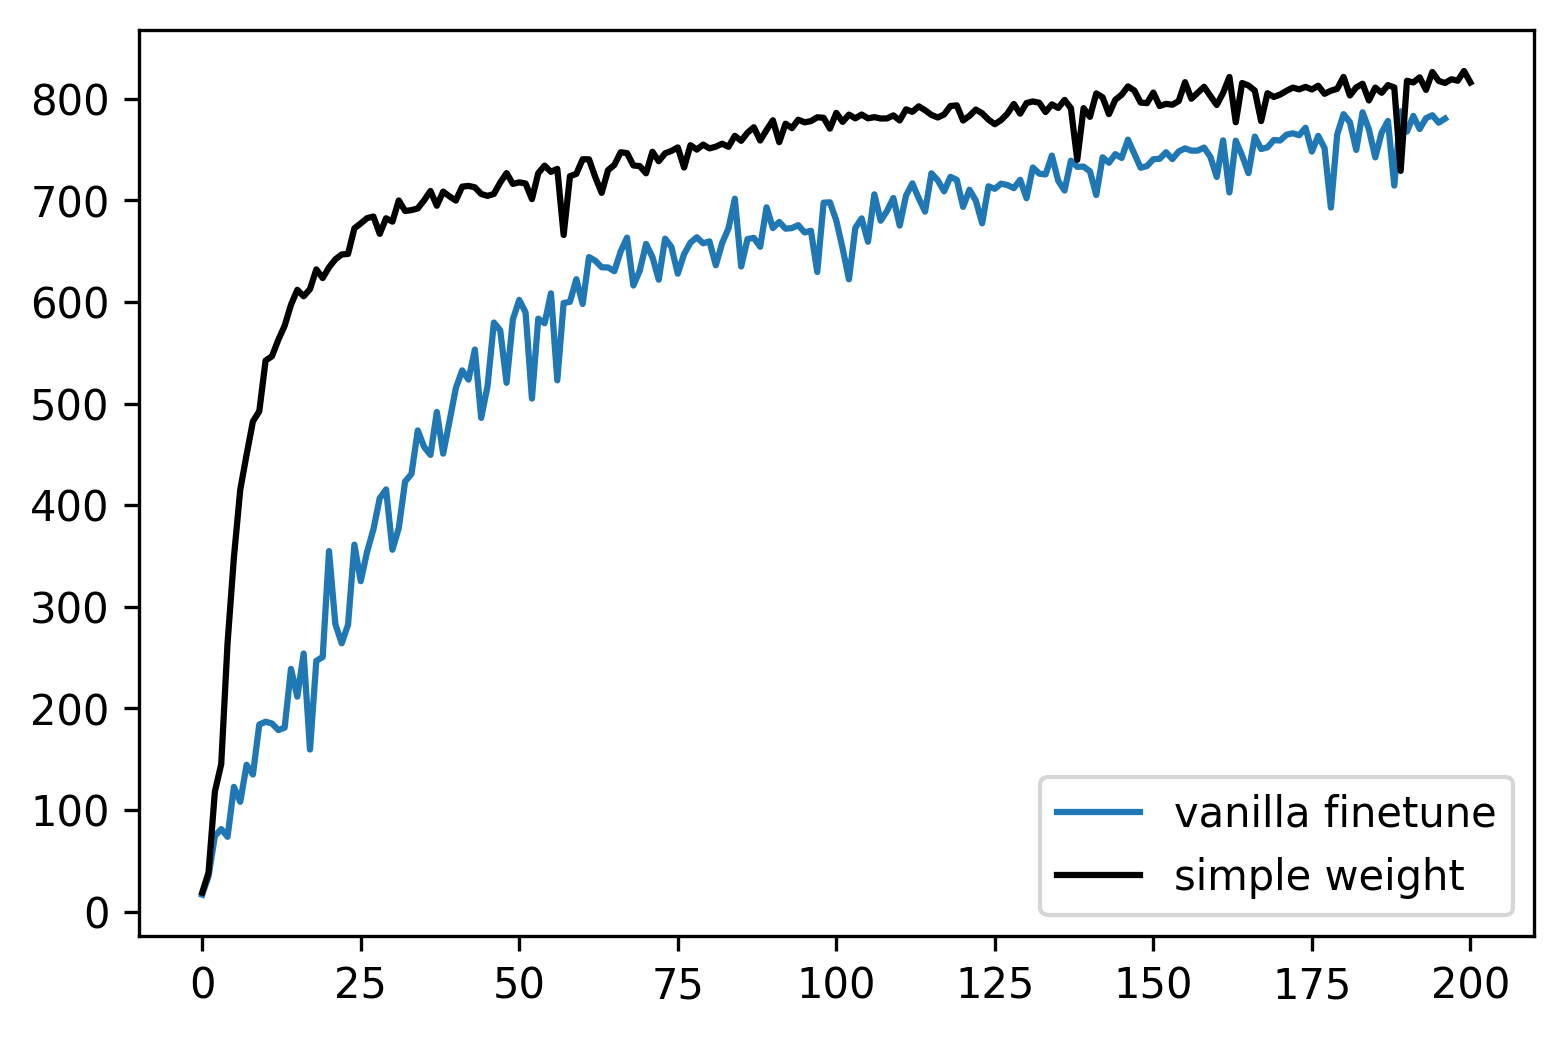
\includegraphics[width=\columnwidth]{Figures/walker_run_simple_weight.png}}
  \caption{Training curves of Walker-Run task from our simple weight agent and vanila DIAYN agent.
  Adding several parameters to help fuse skills helped the agent to learn faster.}
  \label{walker-run-simple-weight}
  \end{center}
  \vskip -0.2in
  \end{figure}


  \begin{figure}[ht]
    \vskip 0.2in
    \begin{center}
    \centerline{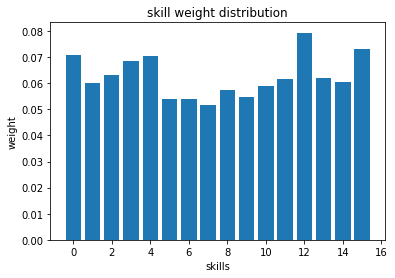
\includegraphics[width=\columnwidth]{Figures/skill_weight.png}}
    \caption{}
    \label{final_skill_weight}
    \end{center}
    \vskip -0.2in
    \end{figure}
Looking at the final learned ${w_i}$, it can be seen that all perspectives are used near evenly.

\subsubsection{Comparison with no skill agent}

We came to a question when we saw that skill weight was evenly distributed.
If we take average of ${[s,z]}$ vectors, isn't it the same as just having state without skill?
This is because the more evenly the importance is distributed, the closer the skill vector is to 0 vector in one-hot vector. Figure needed?
This is because, when concating, the mean of state vector part will be same as the original value,
but the skill vector part will be a near-uniform distributed vector of about $\frac{1}{skilldim}$.
This makes it doubtful whether the skill vector part has any meaning.

If weighted skill vector has really no meaning, then the agent without skill should outperform our method.
Therefore, we compare our method with DDPG + DDPG agent. The result is that our method is better.

This reveals that the skill allows it to learn some meaningful behavior.
Maybe the skill distribution looks like a flat, meaningless vector to our eyes, but the slight difference is meaningful.
If weighted skill vector has really no meaning, then the agent without skill should outperform our method.
Therefore, we compare our method with DDPG + DDPG agent. The result is that our method is better.

This reveals that the skill allows it to learn some meaningful behavior.
Maybe the skill distribution looks like a flat, meaningless vector to our eyes, but the slight difference is meaningful.

\subsection{DIAYN as skill weight predictor}
The second is to use the DIAYN module used in the pretrain phase as a skill weight predictor.
Also, we train DIAYN in end to end manner using DDPG.
DIAYN module was a skill classifier in the pretraining phase, outputting which skill was in charge for the input state.
The final output of DIAYN is logit, which could be easily trasferred to probability when feeded in softmax layer.
We use this probability as a importance weight for skill. 
During the pretraining process, diayn performed the task of predicting skill through the state and we hope 
this pretrain task help diayn module to learn combine skills  to incoming state.

 But the performance was not good. This may be because the pretrain task does not perform a very good weight initializer role,
 or it may be because it is not good to change the weight of skill according to the state.

\subsubsection{Weight transfer from pretrained DIAYN}

\cref*{diayn-as-skill-weight}
In the case of simple weight, skill weight is determined regardless of the incoming state.
However, using the DIAYN module as skill weight predictor creates an association between state and skill weights.
With the transfered weight from pretrained phase, DIAYN module learns to output the skill weight in end to end manner.
However, the learning results were not good.
There was a part where the performance deteriorated significantly for a certain period.

\begin{figure}[ht]
  \vskip 0.2in
  \begin{center}
  \centerline{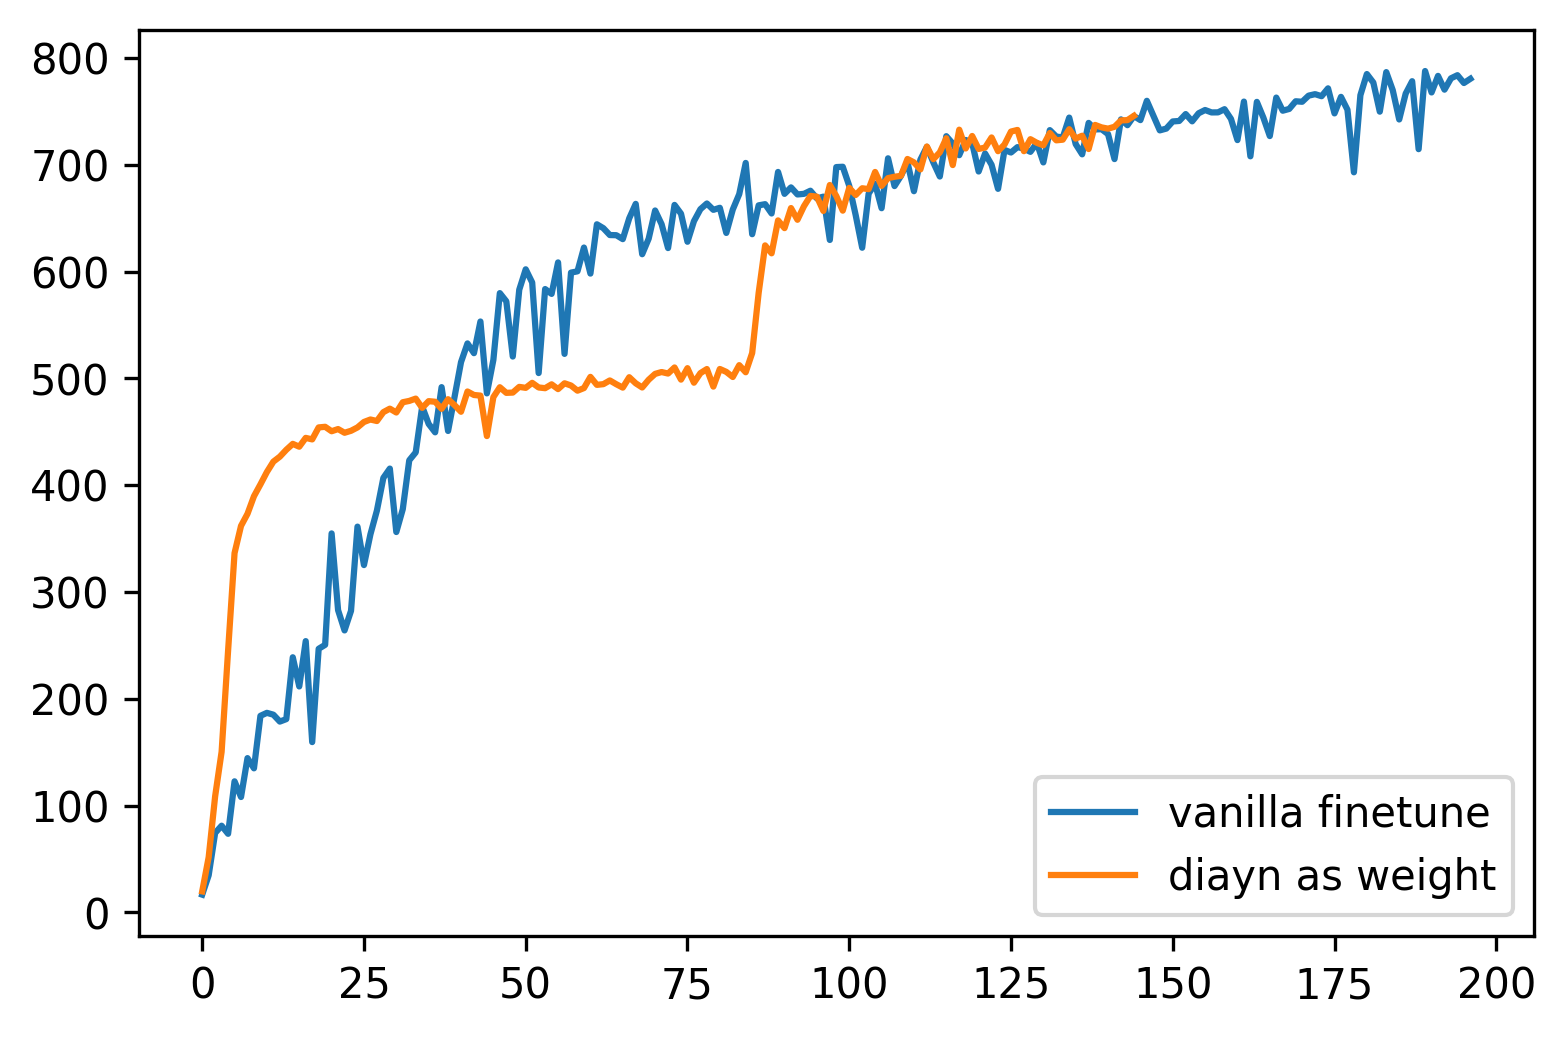
\includegraphics[width=\columnwidth]{Figures/diayn_as_skill_on_walker_run.png}}
  \caption{Historical locations and number of accepted papers for International
  Machine Learning Conferences (ICML 1993 -- ICML 2008) and International
  Workshops on Machine Learning (ML 1988 -- ML 1992). At the time this figure was
  produced, the number of accepted papers for ICML 2008 was unknown and instead
  estimated.}
  \label{diayn-as-skill-weight}
  \end{center}
  \vskip -0.2in
  \end{figure}

\subsubsection{Train from scratch}
Although it recovered later, but even after recovery, it did not show imporoved performance than the baseline and didn't gain sample efficiency from weight transfer.
We thought that DIAYN weight would be a good initializer as a skill weight predictor, the above experiment reveales we are wrong.
Instead, we randomly init the weight with the intention of using it only as a module to determine the appropriate skill weight depending on the state.
The results were rather better than transferred weight.
This shows that the pretrain task was not very helpful in predicting how to fuse the skill together.




\subsection{MultiHeadAttention to attain several skill weight}
Third, we use MultiHeadAttention to have multiple the skill weights.
The result was fine.
However, there is not much gain compared to Simple Weight.
In this case, using simple weights is parameter efficient.

\subsubsection{self attention}
\subsubsection{use state as query attention}





